\section{Uvod}

Bezbednost kriptosistema koji se danas koriste se zasniva na pretpostavci da su jednosmerne funkcije na kojima se zasnivaju teške, to jest da ne postoje algoritmi koji ih rešavaju na klasičnom računaru u polinomijalnom vremenu. Sistemi kao što su RSA i Difi-Helmanova razmena ključeva se zasnivaju na problemima faktorizacije i diskretnog logaritma i za njih se smatra da su teški. Pretpostavka o težini se zasniva na višedecenijskim neuspelim pokušajima da se ovi problemi reše na klasičnom računaru. 

Ako bi bio pronađen algoritam koji u polinomijalnom vremenu rešava probleme faktorizacije ili diskretnog logaritma, sve informacije koje su do sada šifrovane bi postale kompromitovane. Pojava kvantnih računara ovu situaciju čini mogućom. Šor je pokazao da postoje efikasni algoritmi za faktorizaciju i problem diskretnog logaritma na kvantnim računarima \cite{Shor_1997}. Ovo znači da se sa realizacijom kvantnih računara bezbednost kriptosistema gubi. 

Iako još uvek ne postoje kvantni računari, napori da se oni kreiraju su značajni i verovatno će se pojaviti u budućnosti. Zbog toga treba gledati unapred i razvijati kriptosisteme koji će se odupreti napadima od strane algoritama koji se izvršavaju na kvantnim računarima. Veruje se da su kriptografski sistemi zasnovani na heš funkcijama, kodu, rešetkama, jednačinama sa više promenljivih i kriptografija tajnog ključa kvantnorezistentni \cite{postquantumcryptography:2009} \footnote{Strana 1, pasus 3}. Ovo poglavlje će se fokusirati na sisteme zasnovane na rešetkama.

\section{Kvantni računari}

Trenutno postoje različiti predlozi za arhitekturu kvantnog računara koja će prevazići probleme kvantne mehanike i fizička ograničenja. Iz tog razloga se nećemo osvrtati na konkretne aspekte pravljenja kvantnog računara već ćemo se pozabaviti konceptualnim prikazom elemenata jedne takve mašine. 

Kvantni računar se razlikuje od klasičnog po tome što je u svakom trenutku u superpoziciji \footnote{Superpozicija predstavlja linearnu kombinaciju baznih stanja sistema. Kada govorimo o sistemu sa jednim bitom, stanje bi se moglo opisati formulom $ \ket{\psi} = \alpha \ket{0} + \beta \ket{1}$, gde su $\ket{0}$ i $\ket{1}$ bazna stanja sistema.} stanja koja se mogu predsaviti nizom bitova. Jedan bit kvantnog računara se naziva \textit{kubit} (eng. \textit{qubit}) i on opisuje superpoziciju stanja $0$ i $1$. Ovo se može opisati dvodimenzionim Hilbertovim prostorom: $\mathcal{H} = \mathcal{H}_1 = \mathbb{C} \oplus \mathbb{C} \cong \mathbb{C}^2 $, čiju bazu čine vektori $(1, 0) = \ket{0}$ i $(0,1) = \ket{1}$ \cite{postquantumcryptography:2009} \footnote{Strana 20, pasus 2}.

Kako je za opisivanje stanja kvantnog računara sa jednim bitom bio potreban dvodimenzioni prostor, tako će za opisvanje mašine sa $n$ bitova biti potreban prostor dimenzije $2^n$. Ovo se jednostavno postiže tenzorskim proizvodom Hilbertovih prostora: $\mathcal{H}_n = \mathcal{H} \otimes ... \otimes \mathcal{H}$. Baza ovog prostora je tenzorski proizvod pojedinačnih baza, tj $ \ket{i_1...i_n} = \ket{i_1} \otimes ... \otimes  \ket{i_n} $, gde je $i_1...i_n \in \mathcal{I}_n = \{0,1\}^n$ \cite{postquantumcryptography:2009}.

\begin{example}
    Neka je $n=3$, tada je baza prostora:
    \begin{itemize}
        \item[] $\ket{000} = \ket{0} \otimes \ket{0} \otimes \ket{0}$
        \item[] $\ket{001} = \ket{0} \otimes \ket{0} \otimes \ket{1}$
        \item[] $\ket{010} = \ket{0} \otimes \ket{1} \otimes \ket{0}$
        \item[] $\ket{011} = \ket{0} \otimes \ket{1} \otimes \ket{1}$
        \item[] $\ket{100} = \ket{1} \otimes \ket{0} \otimes \ket{0}$
        \item[] $\ket{101} = \ket{1} \otimes \ket{0} \otimes \ket{1}$
        \item[] $\ket{110} = \ket{1} \otimes \ket{1} \otimes \ket{0}$
        \item[] $\ket{111} = \ket{1} \otimes \ket{1} \otimes \ket{1}$.
    \end{itemize}
\end{example}

Kako bi se vršile transformacije stanja, koriste se unitarne transformacije nad Hilbertovim prostorom. One se aproksimiraju kvantnim logičkim kolima (eng. \textit{gates}) iz fiksnog konačnog skupa $\mathcal{G}$. Tada je program na kvantnom računaru sekvenca kola koja vrše izračunavanja nad ulaznim stanjem i daju izlazno. Konkretni skup $\mathcal{G}$ zavisi od implementacije ali treba da bude u stanju da aproksimira transformacije kvantnih stanja uz neku malu grešku \cite{postquantumcryptography:2009}. Da bi se više reklo o uzrocima grešaka prilikom menjanja kvantnih stanja mora se ući u prirodu kvantnih čestica, njihovu nestabilnost i lako padanje pod uticaj okolnih čestica, pa se na to nećemo osvrtati. Treba imati na umu da se greške prilikom izmena stanja dešavaju iz fizičkih razloga.

Kada se izvrši program, kvantno stanje treba prevesti u konkretno stanje reprezentovano nizom bitova. Ovaj proces se zove očitavanje ili merenje (eng. \textit{measuring}) i po prirodi je nedeterministički. Nedeterminizam, takođe, potiče od prirode kvantnih čestica jer se do trenutka očitavanja stanje nalazi u superpoziciji baznih stanja.

Ako je krajnje stanje kvantne mašine $v = \sum_{I \in I_n} \alpha_I \ket{I} $, očitavanje zavisi od raspodele verovatnoća za stanje $s$. Verovatnoća očitavanja stanja $v$ je $P_v(I) = \frac{|\alpha_I|^2}{\sum_{J \in I_n} |\alpha_J|^2} $. \cite{postquantumcryptography:2009} Nakon merenja, sistem kolapsira u izmereno stanje i ponovnim merenjem dobija se isti rezultat.

Na ovako definisanom modelu je Šor \cite{Shor_1997} definisao algoritam koji efikasno rešavaju probleme faktorizacije i diskretnog logaritma. Kada se uspe sa kreiranjem kvantnog računara dovoljne jačine, kriptosistemi zasnovani na ovim funkcijama će postati ranjivi. Zbog toga je neophodno  kreirati sisteme koji su kvantnorezistentni, kao što su sistemi zasnovani na rešetkama.

\section{Rešetke}

Ovo poglavlje posvećeno je rešetkama (engl. \textit{lattices}), koje su se u kriptografiji prvobitno koristile za kriptoanalizu postojećih sistema, dok danas predstavljaju osnovu za konstrukciju novih kriptografskih šema. Bezbednost postkvantnih kriptosistema se zasniva na pretpostavljenoj težini problema na rešetkama kao što su problem najkraćeg vektora i problem najbližeg vektora. Za ove probleme se smatra da ne postoje algoritmi koji ih rešavaju u polinomijalnom vremenu ni na klasičnom ni na kvantnom računaru.

\begin{definition}
    \textbf{Rešetka} $\latt$ je skup celobrojnih linearnih kombinacija linearno nezavisnih vektora $\{b_1, ..., b_m\}, b_i \in \mathbb{R}^n$. Drugim rečima, rešetka $\latt = \{ \sum_{i=1}^m a_ib_i \mid a_i \in \mathbb{Z} \} = \{ B \textbf{a} \mid \textbf{a} \in \mathbb{Z}^n \}$, gde je $B = [b_1, ..., b_m]$ bazna matrica rešetke, a vektori $\{b_1, ..., b_m\}$ čine bazu rešetke.
\end{definition}

Kako je rešetka $\latt$ diskretan skup, može se definisati minimalna dužina nenula vektora $\lambda_1(\latt) := \min \{||x|| \ | x \in \latt, x \neq 0 \} $. Element za koji važi da  mu je dužina jednaka $\lambda_1$ se naziva \textit{najkraći nenula vektor rešetke} i nalaženje ovog elementa se generalno smatra teškim \cite{smart2016cryptography} \footnote{Strana 81, pasus 2}. 

Za rešetku $\latt$ i njenu baznu matricu $B$ možemo definisati \textit{diskriminantu} $\Delta(\latt) = |\det(B^TB)|^{1/2} $, to jest $\Delta(\latt) = |\det(B)|$ ako je $B$ kvadratna matrica. Vrednost diskriminante definiše zapreminu fundamentalnog paralelepipeda koji razapinju bazni vektori \cite{smart2016cryptography}. 

Jedna rešetka ima beskonačan broj baza, pa se može definisati šta je dobra, a šta loša baza za jednu rešetku. \textit{Dobra baza} je ona čiji su vektori kratki i međusobno približno ortogonalni. \textit{Loša baza} se sastoji od relativno dugih vektora između kojih je mali ugao. Na slici \ref{fig:osnovna_rešetka_2d} je prikazana rešetka čija je dobra baza $\{(1,0), (0,1)\}$ jer su vektori međusobno ortogonalni i kratki, a loša $\{(3,0), (5,1)\}$ \cite{meyer2025postquantumcryptographyanalysiscodebased} \footnote{Strana 7, pasus 3}. 

\begin{figure}[h]
    \centering
    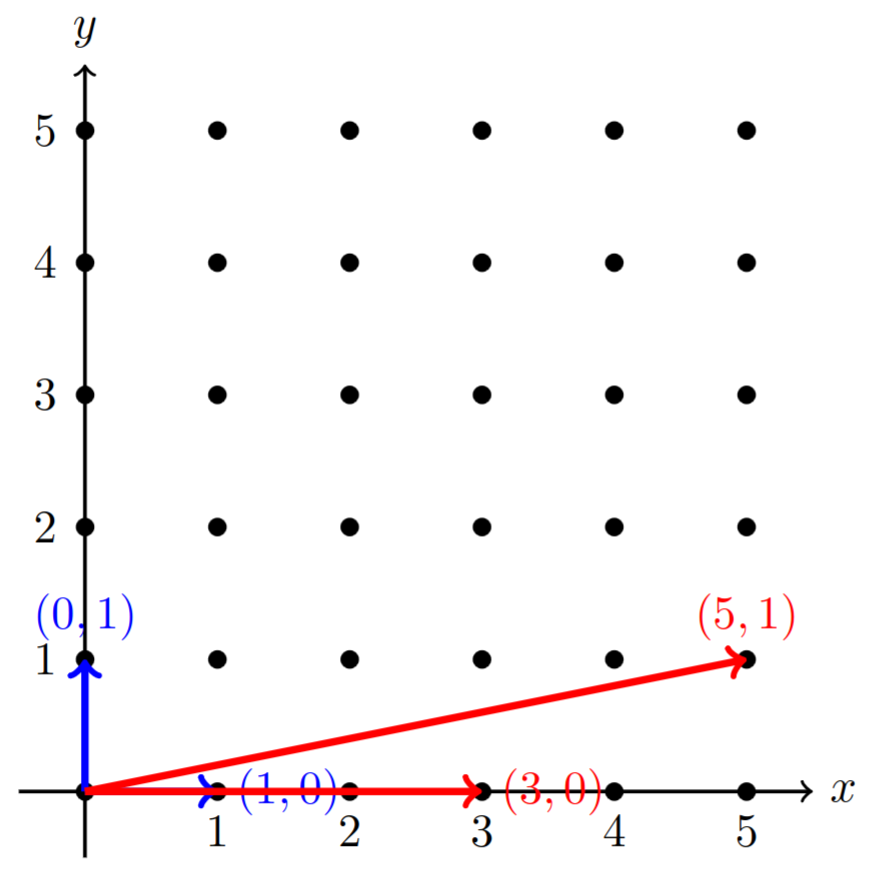
\includegraphics[width=0.5\linewidth]{images/lattices/osnovna_rešetka_2d.png}
    \caption{Struktura rešetke, sa prikazom dobre (plava) i loše (crvena) baze. }
    \label{fig:osnovna_rešetka_2d}
\end{figure}

Za proizvoljnu rešetku $\latt$ čija je baza $B$ se ne može uvek naći potpuno ortogonalna baza, ali postoji \textit{LLL} (Lenstra, Lenstra i Lovász) \textit{algoritam} koji daje redukovanu bazu. On u polinomijalnom vremenu nalazi redukovanu bazu čiji su vektori relativno kratki i približno međusobno ortogonalni, pri čemu je prvi vektor te baze približan najkraćem nenula vektoru rešetke $\latt$, sa faktorom aproksimacije $2^{(n-1)/2}$, gde je $n$ dimenzija kvadratne bazne matrice \cite{smart2016cryptography}.

Poseban tip rešetki su $q$-arne (eng. \textit{q-ary lattice}). Rešetka $\latt$ je $q$-arna ako važi $q \mathbb{Z}^n \subset \latt \subset \mathbb{Z}^n$ za neko celobrojno $q$. Za proizvoljnu matricu $A \in \mathbb{Z}_q^{n \times m}$ mogu se definisati dve $m$-dimenzione $q$-arne rešetke:

\[ \Lambda_q (A) = \{ y \in \mathbb{Z}^m \mid y= A^T z \ \pmod q, z \in \mathbb{Z}^n\}, \]
\[\Lambda_q^{\bot}(A) = \{y \in \mathbb{Z}^m \mid Ay = 0 \pmod q\} \].

Ovaj tip rešetki igra centralnu ulogu u konstrukciji savremenih kriptosistema zasnovanih na rešetkama i biće korišćene u nastavku rada.

\subsection{Teški problemi na rešetkama}

Postoje dva problema na rešetkama koja se smatraju teškim, to su problem najkraćeg vektora i problem najbližeg vektora. Pošto se pretpostavlja da je teško rešiti ove probleme i na klasičnom i na kvantnom računaru, postoje predlozi za postkvantne kriptosisteme koji se zasnivaju na njima. NIST (eng. \textit{National Institute of Standards and Technology}) je 2024. godine objavio standarde za postkvantnu kriptografiju koji se zasnivaju na teškim problemima na rešetkama i dao preporuku da se započne njihova upotreba što pre \cite{niststandard}.

\begin{definition}
    \textbf{Problem najkraćeg vektora (eng. \textit{Shortest Vector Problem - SVP}):} Neka je $\latt$ rešetka čija je baza $B$, tada je problem najkraćeg vektora nalaženje nenula vektora $x \in \latt$ za koji važi $||x|| \leq ||y||$ za svaki nenula vektor $y \in \latt$. Drugim rečima, treba naći $x$ takav da je $||x|| = \lambda_1 (\latt)$.
\end{definition}

Postoje i alternativne definicije ovog problema, kao što je \textbf{aproksimativni problem najkraćeg vektora}, u oznaci SVP$_\gamma$. Ova verzija problema se odnosi na nalaženje vektora $x \in \latt$ takvog da je $||x|| \leq \gamma \cdot \lambda_1 (\latt)$, za neku malu konstantnu $\gamma$. LLL algoritam nam omogućava da nađemo ovu vrstu najkraćeg vektora u rešetki, pri čemu je $\gamma = 2 ^ {(n-1)/2}$ \cite{smart2016cryptography} \footnote{Strana 86, pasus 1}.

Rešenje problema najkraćeg vektora nije jedinstveno jer ako je vektor $x$ njegovo rešenje, onda je i vektor $-x$. Na slici \ref{fig:svp_rešenje} se vidi primer dva najkraća vektora u dvodimenzionalnoj rešetki pri čemu su oni međusobno suprotni vektori.

\begin{figure}[h]
    \centering
    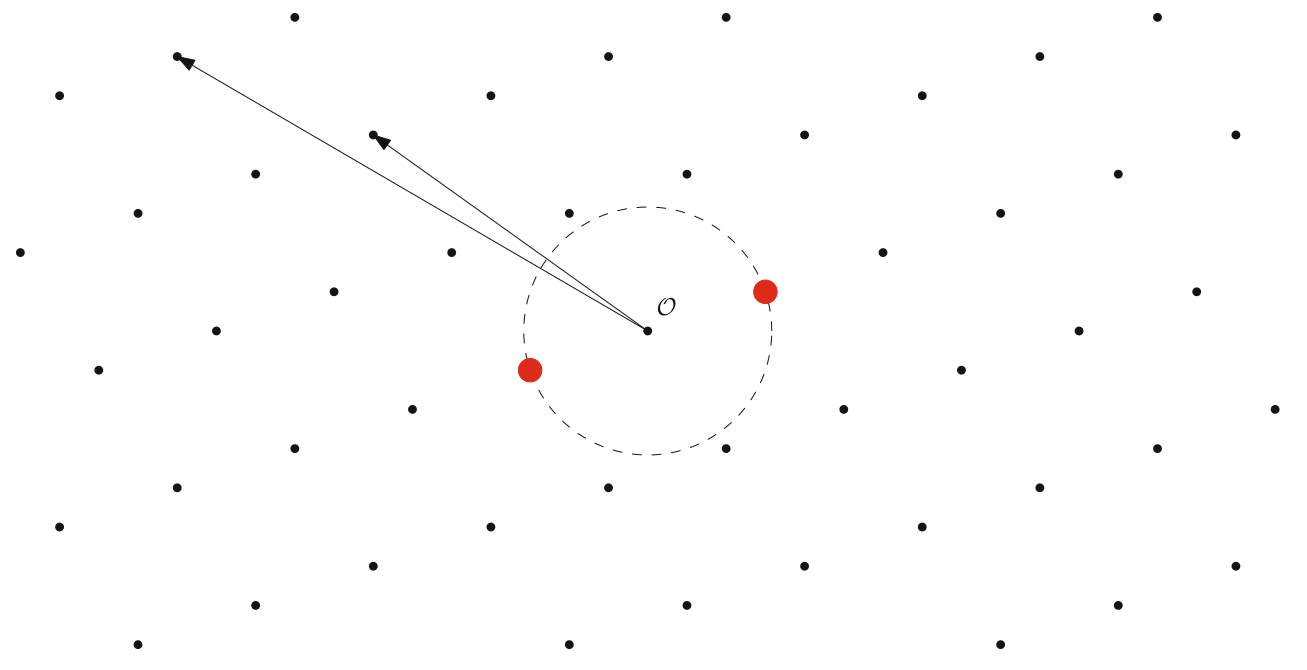
\includegraphics[width=0.75\linewidth]{images/lattices/svp_rešenje.png}
    \caption{Primer rešenja problema najkraćeg vektora u dvodimenzionalnoj rešetki. Crvenom bojom su označeni najkraći vektori, dok su crne strelice bazni vektori.}
    \label{fig:svp_rešenje}
\end{figure}

\begin{definition}
    \textbf{Problem najbližeg vektora (eng. \textit{Closest Vector Problem - CVP})}: Neka je $\latt$ $n$-dimenziona rešetka sa bazom $B$ i $x \in \mathbb{R}^n$ vektor koji ne pripada rešetki, problem najbližeg vektora se sastoji od nalaženja vektora $y \in \latt$ takvog da je $||x-y|| \leq ||x-z||$ za svako $z \in \latt$.
\end{definition}

Kao i kod problema najkraćeg vektora, imamo i aproksimativni problem najbližeg vektora, koji se često označava sa CVP$_\gamma$. Cilj ovog problema je naći $y$ takvo da je $||x-y|| \leq \gamma ||x-z||$ za svaki vektor $z\in \latt$, za neku malu konstantnu vrednost $\gamma$. Na slici \ref{fig:cvp_resenje} se vidi primer jedne dvodimenzionalne rešetke, sa njenim baznim vektorima i vektorom koji je najbliži vektoru koji nije iz rešetke.

\begin{figure}[h]
    \centering
    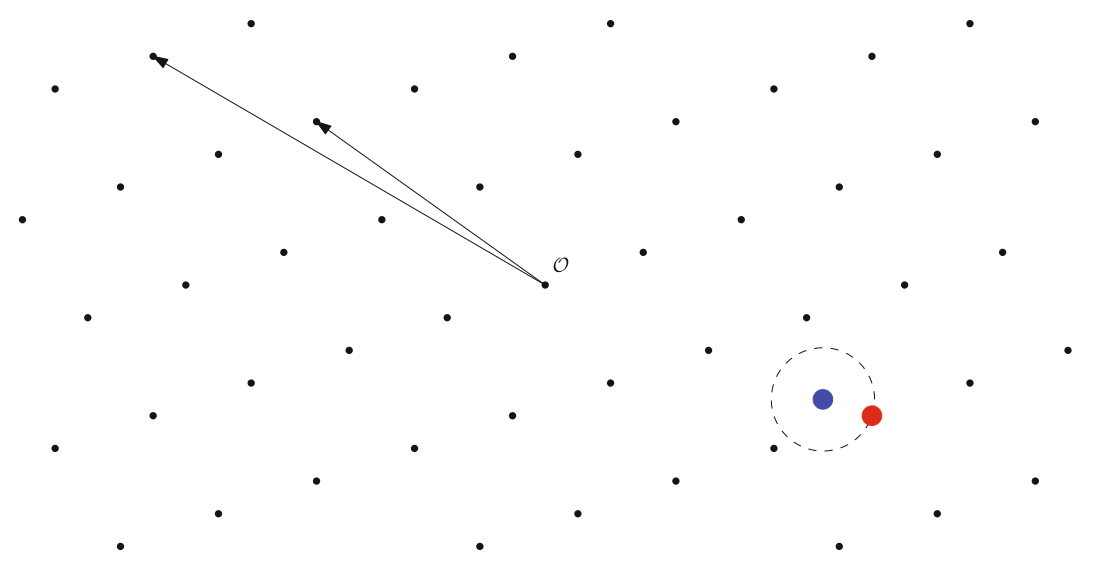
\includegraphics[width=0.75\linewidth]{images/lattices/cvp_rešenja.png}
    \caption{Primer rešenja problema najbližeg vektora u dvodimenzionalnoj rešetki. Crvenom bojom je označen vektor koji pripada rešetki i najbliži je plavo obeleženom vektoru koji joj ne pripada, dok su crne strelice bazni vektori.}
    \label{fig:cvp_resenje}
\end{figure}

%TODO: dodati reference na poglavlja, kada budu napisana
%TODO: proveriti prevod za BDD
Postoji još jedan problem na rešetkama koji je značajan za oblasti učenja sa greškama i potpuno homomorfne enkripcije. Taj problem je \textit{problem dekodiranja na ograničenoj udaljenosti} koji je sličan problemu najbližeg vektora ali sa dodatom informacijom o granici za udaljenost između vektora koji pripada rešetki i onome koji ne pripada.

\begin{definition}
    \textbf{Problem dekodiranja na ograničenoj udaljenosti (eng. \textit{Bounded-Distance Decoding Problem - BDD}) } Neka je $B$ baza rešetke $\latt$ u $n$-dimenzionalnom realnom prostoru i $x\in \mathbb{R}^n$ vektor koji ne pripada rešetki $\latt$. BDD$_\lambda$ problem se odnosi na pronalaženje vektora $y \in \latt$ takvog da je $||x-y|| \leq \lambda \cdot\lambda_1(\latt)$, za realan broj $\lambda$.
\end{definition}

Problemi koji su pomenuti u ovom poglavlju se smatraju teškim za rešavanje i na klasičnom i na kvantnom računaru, to jest ne postoje algoritmi koji ih rešavaju u polinomijalnom vremenu \cite{postquantumcryptography:2009}. Zbog ove osobine predstavljaju dobru osnovu za kreiranje kvantnorezistentnih kriptosistema. 
